\mysection{РАЗРАБОТКА АРХИТЕКТУРЫ ПРОГРАММНОГО ОБЕСПЕЧЕНИЯ}
\subsection{Требования к реализуемой системе}
\label{subsec:build-system-requirements}
Разработка любого ПО должна начинаться с определения требований, которые предоставлены к нему\cite{REQUIREMENTS}.
Так, чтобы определить функциональные требования, нужно проанализировать задачи, на решение которых направлено разрабатываемое программное обеспечение.

Требования к разрабатываемому продукту можно разделить на функциональные и нефункциональные\cite{REQUIREMENTS}.
Функциональные требования определяют, требуемое поведение системы в определенных условиях.
Нефункциональные требования определяют свойства или особенности, которым должна обладать система, или ограничение, которому должна соблюдать система.
Другими словами, требования, отличные от функциональных, могут описывать не что система делает, а как хорошо она это делает\cite{REQUIREMENTS}.

Ниже приведены наиболее важные идеи, задачи и требования, предъявляемые к разрабатываемому продукту.
К системе сборки были поставлены следующие функциональные требования:
\begin{itemize}
  \item кроссплатформенность;
  \item возможность вручную конфигурировать необходимые предустановленные в образ пакеты;
  \item возможность одновременной сборки нескольких образов: минимального, серверного, расширенного;
  \item наличие загрузчика в образах;
  \item наличие пакетного менеджера в образах;
  \item пригодность для использования образов во время разработки ВС;
\end{itemize}
\newpage

\newpage
\subsection{Проектирование системы}
Для построения архитектуры системы сборки необходимо поэтапно рассмотреть процедуру создания образа.

\begin{figure}[h!]
  \centering
  \setlength{\fboxsep}{5pt}
  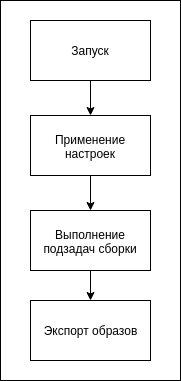
\includegraphics[height=8cm]{build/images/common_build}
  \caption{Этапы создания образа}\label{fig: common_build}
\end{figure}

Кроме того, исходя из требований к системе сборки, важно отметить что полученное решение должно быть кроссплатформенным.
Так, чтобы обеспечить выполнение этого требования предлагается модифицировать общую архитектуру системы с использованием виртуализации на уровне операционной системы(контейнеризации):

\begin{figure}[h!]
  \centering
  \setlength{\fboxsep}{5pt}
  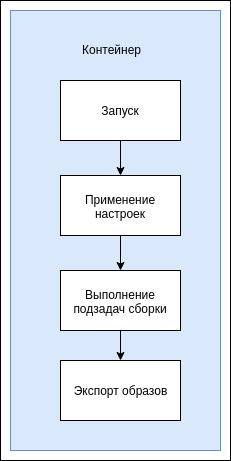
\includegraphics[height=8cm]{build/images/container_build}
  \caption{Архитектура с использованием контейнризации}\label{fig: container_build}
\end{figure}

\newpage
\subsubsection{Этап запуска системы}

Начальным этапом создания образа является заупск системы сборки (рис.~\ref{fig: build_start}).
  На этом этапе система должна выполнить проверку среды исполнения, удостовериться в наличии прав суперпользователя, а также поизвести считывание параметров из конфигурационного файла.
  \begin{figure}[h!]
    \centering
    \setlength{\fboxsep}{5pt}
    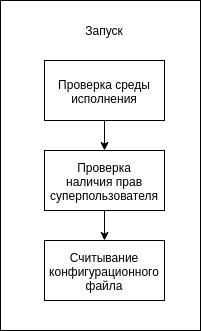
\includegraphics[height=8cm]{build/images/build_start}
    \caption{Запуск системы сборки}\label{fig: build_start}
  \end{figure}

\newpage
\subsubsection{Этап применения настроек}
Применение настроек из конфигурационного файла (рис.~\ref{fig: apply}). На этом этапе система должна выполнить экспорт глобальных констант для сборки.
Кроме того система устанавливает флаги игнорирования стадий сборки и игнорирования стадий экспорта для образа.
\begin{figure}[h!]
  \centering
  \setlength{\fboxsep}{5pt}
  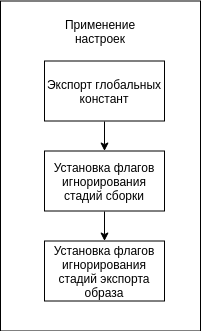
\includegraphics[height=8cm]{build/images/apply}
  \caption{Применение настроек из конфигурационного файла}\label{fig: apply}
\end{figure}

\newpage
\subsubsection{Этап выполнения подзадач}
Выполнение подзадач сборки (рис.~\ref{fig: subtask}). На этом этапе система выполняет prerun-шаг, а после этого производит выполнение подшагов от 00 до 99.
\begin{figure}[h!]
  \centering
  \setlength{\fboxsep}{5pt}
  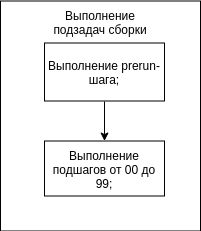
\includegraphics[height=8cm]{build/images/subtask}
  \caption{Выполнение подзадач сборки}\label{fig: subtask}
\end{figure}

\newpage
\subsubsection{Этап экспорта образов}
Экспорт образов (рис.~\ref{fig: export}). На этом этапе система выполняет ряд завершающих и обязательных действий среди которых разметка файла образа,
установка основных пакетов, ядра Linux, загрузчика. После чего производит сохранение образа.
\begin{figure}[h!]
  \centering
  \setlength{\fboxsep}{5pt}
  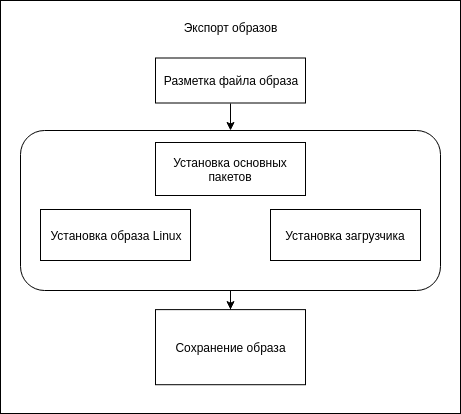
\includegraphics[height=8cm]{build/images/export}
  \caption{Экспорт образов}\label{fig: export}
\end{figure}
\newpage
